\documentclass[a4paper,12pt]{article}
%----------------------PACKAGES----------------------%

% Fonts, Typography, and Text Formatting
\usepackage[charter, cal=cmcal]{mathdesign}      % Charter font and math fonts
\usepackage[scaled=.96]{XCharter}                % Scaled Charter text font
\usepackage{microtype}                           % Fine typographical adjustments (e.g., kerning)

% Colors
\usepackage{xcolor}                              % For defining and using colors

% Math Tools and Symbols
\usepackage{amsmath}                             % Core package for advanced math typesetting
\usepackage[fixamsmath]{mathtools}               % Extensions to amsmath, fixing bugs and adding features
% \usepackage{nicematrix}                        % Create matrices with enhanced formatting options
\usepackage{bm}                                  % Bold math symbols
\usepackage[Smaller]{cancel}                     % Cancel terms in equations with diagonal lines
\usepackage[e]{esvect}                           % Extended vector arrows
\usepackage{siunitx}                             % For formatted units

% Lists, Tables, and Layout Utilities
% \usepackage{booktabs}                          % Professional-quality tables
\usepackage{tabularray}                          % Improves and add to base table functionality 
\usepackage[shortlabels, inline]{enumitem}       % Customized lists with inline option
% \usepackage{parskip}                           % Adjust paragraph spacing (removes indent and adds space between paragraphs)

% Page Layout and headers
% \usepackage{geometry}                          % Adjust page layout (margins, etc.)
% \usepackage{fancyhdr}                          % Custom headers and footers
% \usepackage{titling}                           % Customize title formatting
% \usepackage{scrlayer-scrpage}                    % KOMA-script enhanced headers and footers support

% Floating Figures and Tables
\usepackage{float}                               % Control the placement of figures and tables

% Graphics and Plotting 
\usepackage{tikz}                                % Drawing and diagramming
\usepackage{pgfplots}                            % Create plots using TikZ
\pgfplotsset{compat=1.18}

% Miscellaneous 
% \usepackage{lipsum}                            % Generate placeholder text
 
\usepackage{expl3}
%----------------------DELIMITERS----------------------%

\makeatletter
\NewDocumentCommand \NewPairedDelimiter { m m m } {%
  \expandafter\DeclarePairedDelimiter\csname PAIRED\string#1\endcsname{#2}{#3}%
  \newcommand#1{%
    \@ifstar{\csname PAIRED\string#1\endcsname}
            {\@ifnextchar[{\csname PAIRED\string#1\endcsname}
                          {\csname PAIRED\string#1\endcsname*}%
            }%
  }%
}
\NewDocumentCommand \NewPairedDelimiterX { m m m m } {%
  \expandafter\DeclarePairedDelimiterX\csname PAIREDX\string#1\endcsname[2]{#2}{#3}{#4}%
  \newcommand#1{%
    \@ifstar{\csname PAIREDX\string#1\endcsname}
            {\@ifnextchar[{\csname PAIREDX\string#1\endcsname}
                          {\csname PAIREDX\string#1\endcsname*}%
            }%
  }%
}
\NewDocumentCommand \NewPairedDelimiterXPP { m m m m m m } {%
  \expandafter\DeclarePairedDelimiterXPP\csname PAIREDXPP\string#1\endcsname[2]{#2}{#3}{#4}{#5}{#6}%
  \newcommand#1{%
    \@ifstar{\csname PAIREDXPP\string#1\endcsname}
            {\@ifnextchar[{\csname PAIREDXPP\string#1\endcsname}
                          {\csname PAIREDXPP\string#1\endcsname*}%
            }%
  }%
}
\makeatother

\NewPairedDelimiterXPP \map {#1} ( ) { } { #2 } 

\NewPairedDelimiterXPP \bmap {#1} [ ] { } { #2 }

\NewPairedDelimiterXPP \cmap { #1 } \{ \} { } { #2 }


\NewPairedDelimiter \parens ( )

\NewPairedDelimiter \bracks [ ] 

\NewPairedDelimiter \curls \{ \} 

\NewPairedDelimiter \abs \lvert \rvert 

\NewPairedDelimiter \norm \lVert \rVert

\NewPairedDelimiter \floor \lfloor \rfloor

\NewPairedDelimiter \ceil \lceil \rceil

\NewPairedDelimiterX \ff . . { #1 \delimsize/ #2 } 


%----------------------VECTORS & BOLDING----------------------%

\let\vvv\vv 
\def\vv#1{\vvv{\vb{#1}}}

\NewDocumentCommand \vb { s m } { 
    \IfBooleanTF { #1 } { \mathbf{ #2 } } { \boldsymbol{ #2 } } 
}

\NewDocumentCommand \vu { s m } {
     \widehat { \IfBooleanTF {#1} { \boldsymbol } { \mathbf } {#2} } 
}

\NewDocumentCommand \vc { s m }{ 
    \widehat { \IfBooleanTF {#1} { \mathbf } { \boldsymbol } {#2} } \,
}

\NewDocumentCommand \cross { } { 
    \boldsymbol{\times} 
}

\NewDocumentCommand \vdot { } { 
    \boldsymbol{\cdot} 
}

\NewDocumentCommand \grad { } { 
    \vv \nabla 
}

\RenewDocumentCommand \div { } { 
    \grad \vdot 
}

\NewDocumentCommand \curl { } { 
    \grad \cross 
}

\NewDocumentCommand \lap { O{2} } {
    \nabla^{#1}
}

%----------------------DERIVATIVES----------------------%

\NewDocumentCommand \diff { } {
    \mathord{d\mkern-0.4\thinmuskip}
}
\NewDocumentCommand \pdiff { } {
    \partial\mkern-0.5\thinmuskip
}
\NewDocumentCommand \dd { } {
    \mathop{}\!\diff
}

\NewDocumentCommand \dv { s O{} m } {
		\IfBooleanTF {#1} { \ff } { \f }
		{ \diff #2 } { \diff #3 }
}

\NewDocumentCommand \ndv { m s O{} m } {
		\IfBooleanTF {#2} { \ff* } { \f }
		{ \diff^{#1} #3 } { \diff #4^{#1} }
}

\NewDocumentCommand \pndv { m s O{} m } {
		\IfBooleanTF {#2} { \ff* } { \f }
		{ \pdiff^{#1} #3 } { \pdiff #4^{#1} }
}
\NewDocumentCommand \pdv { s O{} m } {
		\IfBooleanTF {#1} { \ff* } { \f }
		{ \pdiff #2 } { \pdiff #3 }
}

\NewDocumentCommand \pddv { s O{} m m } {
		\IfBooleanTF {#1} { \ff* } { \f }
		{ \pdiff^2 #2 } { \pdiff #3 \pdiff #4 }
}

\NewDocumentCommand \pdddv { s O{} m m m } {
		\IfBooleanTF {#1} { \ff* } { \f }
		{ \pdiff^3 #2 } { \pdiff #3 \pdiff #4 \pdiff #5 }
}

%----------------------MISC. MATH MACROS----------------------%


\NewDocumentCommand \Implies { } {
     \;\Rightarrow
}

\NewDocumentCommand \Iff { } {
     \; \Leftrightarrow \;
}

\NewDocumentCommand \rect { } {
     \op{rect}
}

\RenewDocumentCommand \Re { } {
    \op{Re}    
}

\RenewDocumentCommand \Im { } {
    \op{Im}    
}

\NewDocumentCommand \csch { } {
\op{csch}
}

\NewDocumentCommand \sech { } {
\op{sech}
}

\NewDocumentCommand \trans { m } {
    #1^{\mathsf T}
}

\NewDocumentCommand \comp { m } {
    #1^{\mathsf C}
}

\NewDocumentCommand \adj { m } {
    #1^{\mathsf H}
}


\NewDocumentCommand \mat { O{p} o +m }
	{
		\IfValueTF {#2}
			{ \begin{#1matrix*}[#2] }
			{ \begin{#1matrix} }
			#3
		\IfValueTF {#2}
			{ \end{#1matrix*} }
			{ \end{#1matrix} }
	}
    
%----------------------MISC. TEXT MACROS----------------------%

% Define date formats
\makeatletter
\newcommand*\twodigits[1]{\ifnum#1<10 0\fi\the#1}
\newcommand*\shortdate{\the\year-\twodigits\month-\twodigits\day}
\newcommand*\monthyear{%
    \ifcase\month\or January\or February\or March\or April\or May\or June\or
  July\or August\or September\or October\or November\or
  December\fi\space\number\year
}
\makeatother

\RenewCommandCopy \t {
    \text
}

%----------------------SHORTCUTS----------------------%

\NewCommandCopy \f {
    \frac
}

\RenewCommandCopy \le {
    \leqslant
}

\RenewCommandCopy \ge {
    \geqslant
}

\NewCommandCopy \tb {
    \textbf
}

\NewCommandCopy \ds {
    \displaystyle    
}

\NewCommandCopy \op {
    \operatorname    
}

\NewCommandCopy \eps {
    \varepsilon
}

\NewCommandCopy \q {
    \quad
}

\NewCommandCopy \vd {
    \vdot
}

\NewCommandCopy \qq {
    \qquad
}

\NewCommandCopy \0 {
    \mathcolor
}

\NewCommandCopy \1 {
    \indicator
}

\NewCommandCopy \2 {
    \cdot
}

\NewCommandCopy \3 {
    \sqrt
}

\NewCommandCopy \4 {
    \frac
}

\NewCommandCopy \5 {
    \ff
}

\NewCommandCopy \6 {
    \map
}

\NewCommandCopy \7 {
    \bmap
}

\NewCommandCopy \8 {
    \parens
}

\NewCommandCopy \9 {
    \bracks
}
%----------------------COLOURS----------------------%


%----------------------TYPESET----------------------%
% Commands for \mathbb

\newcommand{\N}{\vb*{N}}
\newcommand{\Q}{\vb*{Q}}
\newcommand{\R}{\vb*{R}}
\newcommand{\Z}{\vb*{Z}}
\newcommand{\C}{\vb*{C}}
\newcommand{\F}{\vb*{F}}

% Commands for \mathcal

\renewcommand{\AA}{\mathcal{A}}
\newcommand{\BB}{\mathcal{B}}
\newcommand{\CC}{\mathcal{C}}
\newcommand{\DD}{\mathcal{D}}
\newcommand{\EE}{\mathcal{E}}
\newcommand{\FF}{\mathcal{F}}
\newcommand{\GG}{\mathcal{G}}
\newcommand{\HH}{\mathcal{H}}
\newcommand{\II}{\mathcal{I}}
\newcommand{\JJ}{\mathcal{J}}
\newcommand{\KK}{\mathcal{K}}
\newcommand{\LL}{\mathcal{L}}
\newcommand{\MM}{\mathcal{M}}
\newcommand{\NN}{\mathcal{N}}
\newcommand{\OO}{\mathcal{O}}
\newcommand{\PP}{\mathcal{P}}
\newcommand{\QQ}{\mathcal{Q}}
\newcommand{\RR}{\mathcal{R}}
\renewcommand{\SS}{\mathcal{S}}
\newcommand{\TT}{\mathcal{T}}
\newcommand{\UU}{\mathcal{U}}
\newcommand{\VV}{\mathcal{V}}
\newcommand{\WW}{\mathcal{W}}
\newcommand{\XX}{\mathcal{X}}
\newcommand{\YY}{\mathcal{Y}}
\newcommand{\ZZ}{\mathcal{Z}}

% Commands for \mathscr
\newcommand{\AAA}{\mathscr{A}}
\newcommand{\BBB}{\mathscr{B}}
\newcommand{\CCC}{\mathscr{C}}
\newcommand{\DDD}{\mathscr{D}}
\newcommand{\EEE}{\mathscr{E}}
\newcommand{\FFF}{\mathscr{F}}
\newcommand{\GGG}{\mathscr{G}}
\newcommand{\HHH}{\mathscr{H}}
\newcommand{\III}{\mathscr{I}}
\newcommand{\JJJ}{\mathscr{J}}
\newcommand{\KKK}{\mathscr{K}}
\newcommand{\LLL}{\mathscr{L}}
\newcommand{\MMM}{\mathscr{M}}
\newcommand{\NNN}{\mathscr{N}}
\newcommand{\OOO}{\mathscr{O}}
\newcommand{\PPP}{\mathscr{P}}
\newcommand{\QQQ}{\mathscr{Q}}
\newcommand{\RRR}{\mathscr{R}}
\newcommand{\SSS}{\mathscr{S}}
\newcommand{\TTT}{\mathscr{T}}
\newcommand{\UUU}{\mathscr{U}}
\newcommand{\VVV}{\mathscr{V}}
\newcommand{\WWW}{\mathscr{W}}
\newcommand{\XXX}{\mathscr{X}}
\newcommand{\YYY}{\mathscr{Y}}
\newcommand{\ZZZ}{\mathscr{Z}}




\usepackage{anysize}
\marginsize{2cm}{2cm}{1cm}{2cm}
\usepackage{fancyhdr}
\setlength{\headheight}{14.5pt}
\renewcommand{\headrulewidth}{0pt}
\usepackage{soul}
\usepackage[dvipsnames]{xcolor}
\usepackage{hyperref}
\hypersetup{
    colorlinks=true,
    linkcolor=black,
    citecolor=CadetBlue,
    filecolor=CadetBlue,
    urlcolor=CadetBlue
}

\usepackage{lipsum}
\usepackage{multicol}
\usepackage{parskip}

\setlength\columnsep{18pt}

% Sets abstract
\renewenvironment{abstract}
 {\par\noindent\textbf{\abstractname}\ \ignorespaces}
 {\par\noindent\medskip}

\begin{document}

% Makes header
\pagestyle{fancy}
\thispagestyle{empty}
\fancyhead[R]{\textit{Qalam}}
\fancyhead[L]{}

% Makes footnotes with an asterisk
\renewcommand*{\thefootnote}{\fnsymbol{footnote}}

\begin{center}
    \Large{\textbf{Comparison of Ray Optics and Wave Optics in Imaging Systems}}
    \vspace{0.5cm}
 
    \normalsize
    \ Abdullah Qalam, Abdellatif Mohamed Ahmed, Areeba Warsi
    \vspace{0.1cm}
 
    \textit{Ozyegin University}
    \medskip
 
    \normalsize
\end{center}

{\color{gray}\hrule}
\vspace{0.4cm}

\begin{abstract}
    This paper aims to provide a comparative analysis of ray (geometric) optics with wave (physical) optics in the context of 
imaging systems. We evaluate how well each explains or predicts how images are formed and what limits the quality of those images in physical optical systems.   
More specifically, we highlight: 
\begin{itemize}
    \item Limitations of the ray model in representing physical phenomena accurately.
    \item How the wave model explains phenomena that affect image sharpness, brightness, and contrast.
\end{itemize}
To that end, we consider the following two points of interest under different optical setups by means of a simulation-based approach, and verify
whether the respective ray and wave models' predictions hold:  
\begin{enumerate} 
    \item Diffraction Effects in a Lens-Based Imaging System.
        \begin{itemize}
            \item \tb{Setup:} Simulate a point source imaged through a circular lens aperture. 
            \item \tb{Ray Optics Prediction:} The image of a point is a perfect point at the focus.
            \item \tb{Wave Optics Prediction:} The image is an Airy disk due to diffraction at the aperture edges.
        \end{itemize}
    \item Aberrations in High-Aperture Lenses.
        \begin{itemize}
            \item \tb{Setup:} Simulate off-axis point imaging using a high numerical aperture lens, for simplicity, a spherical lens is considered. 
            \item \tb{Ray Optics Prediction:} Rays don't all focus to a single point due to primarily spherical and chromatic aberration, but can still be traced.
            \item \tb{Wave Optics Prediction:} Also accounts for the interference patterns and phase shifts that occur; blurring and PSF distortions should be more precise. 
        \end{itemize}
\end{enumerate}
The above two setups support our objectives by examining two important optical processes: diffraction and aberrations, both of which critically impact optical system performance. Our simulations confirm 
our predictions for both models and reveal the limitations of the ray model in predicting systems with strong diffractive or aberrative effects.   


\end{abstract}

{\color{gray}\hrule}
\medskip
\newpage

\begin{multicols}{2}
    \tableofcontents
    \section{Introduction}
    \lipsum
\end{multicols}

{\color{gray}\hrule}
\begin{center}
\section{Theory and Literature Review}
\bigskip
\end{center}
{\color{gray}\hrule}
\begin{multicols}{2}
\subsection{Fundamental Equations and Models}
Ray optics simplifies light behavior by modeling it as straight-line rays and neglecting diffraction and interference,
as discussed previously. The model is governed by Fermat's Principle, which states that light follows the path of least time.
From this, fundamental geometric rules like Snell's Law for refraction arise: 
\[
n_1\6\sin{\theta_1} = n_2\6\sin{\theta_2}
\]
Under small-angle (paraxial) conditions, ray propagation through optical components can be described using ray transfer matrices (ABCD matrices): \[
\begin{bmatrix}
x_2 \\ \theta_2
\end{bmatrix} = \begin{bmatrix} A & B \\ C & D \end{bmatrix} \begin{bmatrix} x_1 \\ \theta_1 \end{bmatrix} 
\]
On the other hand, wave optics treats light as a wave, enabling accurate modeling of phenomena such as interference and diffraction,
which are especially important when feature sizes are comparable to the wavelength of light. 
One key application of wave optics is in understanding the point spread function (PSF), 
how a point source of light is imaged through an optical system.

For a circular aperture, the intensity distribution in the image plane is described by the Airy pattern, given by:
\[ 
I(r) = I_0\8{\4{2J_1(kr)}{kr}}^2
\]
This function arises from the Fourier transform of a circular aperture, and it accurately predicts the Airy disk and its 
surrounding diffraction rings, which define the resolution limit of the optical system. This contrasts with ray optics,
which would predict a perfect point image in the absence of aberrations.


\end{multicols}

{\color{gray}\hrule}
\begin{center}
\section{Methodology}
\bigskip
\end{center}
{\color{gray}\hrule}
\begin{multicols}{2}
This study employs simulation-based analysis to investigate and compare the behavior of ray and wave optics in two specific imaging configurations: diffraction through a circular aperture and off-axis imaging with a high-aperture spherical lens. 
The simulations were implemented in Python, and all parameters were normalized where appropriate to emphasize physical
 effects without computational bias. The theoretical setups for each experiment follow the configurations detailed in the appendix.

\subsection{Ray Optics Simulation}

In the ray optics approach, light is modeled as straight lines obeying geometric rules. 
The simulations make use of Snell's law and ray propagation through lenses using paraxial approximations. 
Two cases were examined:

\begin{itemize}
\item \textbf{Diffraction-Limited Focus Without Aberrations:} Rays are emitted from a point source and traced through an ideal thin lens. 
The rays converge perfectly at the geometric focus, and no wave-like behavior such as diffraction or interference 
is considered. This represents the idealized case predicted by geometric optics.

\item \textbf{Aberrated Off-Axis Imaging:} Rays from a point source located off the optical axis are propagated
through a high numerical aperture (NA) spherical lens. Due to the curvature of the lens and the off-axis origin, 
the rays fail to converge to a single point, revealing classical spherical aberration. The resulting spot diagram 
illustrates ray spread and loss of resolution.
\end{itemize}

\subsection{Wave Optics Simulation}

The wave optics framework models light as an electromagnetic wave governed by the scalar diffraction theory. 
To account for diffraction and interference, the angular spectrum and Fourier optics approach were used. 
The simulations explored the following:

\begin{itemize}
\item \textbf{Diffraction through a Circular Aperture:} A monochromatic point source is passed through a circular aperture. The resulting point spread function (PSF) is calculated using the Fraunhofer diffraction integral, which in the far-field limit reduces to the Airy pattern:

\[
I(r) = I_0 \8{\frac{2J_1(kr)}{kr}}^2
\]

where $J_1$ is the first-order Bessel function, $k = \frac{2\pi}{\lambda}$, and $r$ is the radial distance in the image plane. 
This model predicts the central bright disk and surrounding diffraction rings.

\item \textbf{Aberrations in High-NA Lens:} A wavefront with a phase distortion, corresponding to spherical aberration, is propagated through a lens aperture. The aperture function includes a phase delay term of the form:

\[
P(r) = A(r) \exp\left(i k W(r)\right)     
\]

where $W(r)$ represents the aberration function and $A(r)$ the amplitude profile across the aperture. The resulting PSF is computed using a two-dimensional Fourier transform, which reveals distortions and asymmetry in the focal intensity distribution due to interference and phase errors.
\end{itemize}

All simulations were executed using discretized spatial grids and FFT-based propagation techniques, which enabled efficient modeling of diffraction and aberration phenomena. The results were visualized to directly compare the predictions from ray and wave optics under matched conditions.
\end{multicols}

{\color{gray}\hrule}
\begin{center}
\section{Results and Discussion}
\bigskip
\end{center}
{\color{gray}\hrule}
\begin{multicols}{2}
We now go ahead with exploring and discussing the results of our simulations. Each result is shown with the visual outputs from the respective Python simulation, and is followed
by a discussion that compares these findings with theoretical expectations and evaluates the performance of ray and wave
models.
\subsection{Scenario 1: Diffraction-Limited Imaging of a Point Source}
\subsubsection{Ray Optics simulation}
As predicted by the lens maker's equation, all paraxial rays converged at the back focal plane, forming a geometrically
perfect image point. This is illustrated in Figure~\ref{fig:ray-focus}, where the traced rays intersect cleanly on the
optical axis at the image plane.

\begin{figure}[H]
    \centering
    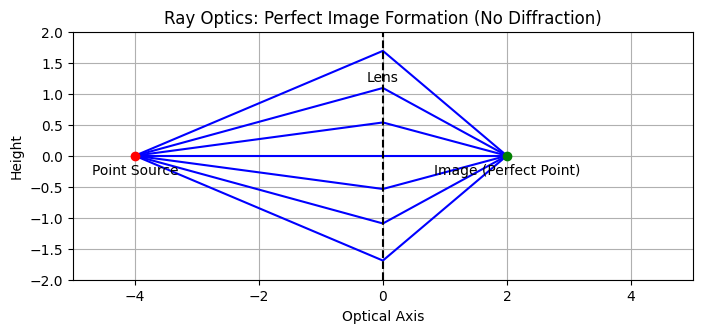
\includegraphics[width=0.45\textwidth]{../images/ray_optics_perfect_focus.png}
    \caption{Ray optics simulation of perfect image formation through a convex lens.}
    \label{fig:ray-focus}
\end{figure}

\subsubsection{Wave Optics Simulation}
Wave optics was then used to evaluate the same configuration. Modeling the lens aperture as a circular pupil,
the propagated field formed an Airy disk pattern due to diffraction. As shown in Figure~\ref{fig:wave-diffraction},
the intensity distribution exhibits a central bright lobe surrounded by concentric rings (although the intensity drops too low for them to be seen beyond the 2nd ring), a clear manifestation of the point
spread function (PSF). The 2D image and the horizontal cross-section intensity profile both highlight this effect.

\begin{figure}[H]
    \centering
    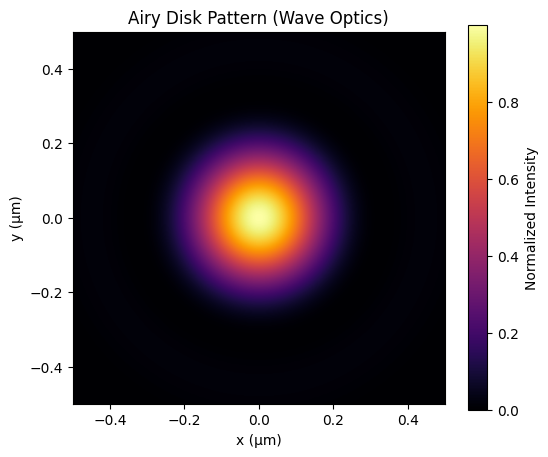
\includegraphics[width=0.45\textwidth]{../images/wave_optics_airy_disk.png}
    \caption{Wave optics simulation showing the Airy disk resulting from a circular aperture.}
    \label{fig:wave-diffraction}
\end{figure}

\subsection{Scenario 2: Aberrations in High-Aperture Lenses}

\subsubsection{Ray Optics Simulation}

In the second setup, an off-axis point source was imaged using a spherical lens with a high numerical aperture.
In the ray-based simulation (Figure~\ref{fig:ray-aberration}), rays that entered the lens at higher angles failed to converge at the same point as the central rays. This introduced spherical aberration,
resulting in a loss of resolution. The simulation captures the deviation of marginal rays and the mismatch at the focal region quite well.

\begin{figure}[H]
    \centering
    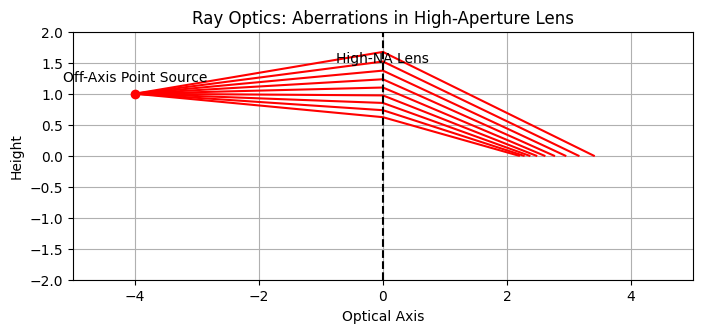
\includegraphics[width=0.45\textwidth]{../images/ray_optics_aberration.png}
    \caption{Ray optics simulation of aberration effects in high-aperture lens systems.}
    \label{fig:ray-aberration}
\end{figure}

\subsubsection{Wave Optics Simulation}

Wave optics simulation was then used to investigate the same aberrated system.
As shown in Figure~\ref{fig:wave-aberration}, the resulting PSF is significantly distorted compared to the ideal Airy disk shown before.
Off-axis field contributions interfere destructively and constructively across the aperture, leading to intensity shifts
and asymmetric blurring. These effects align well with 0ur theoretical expectations for aberration-induced phase errors.

\begin{figure}[H]
    \centering
    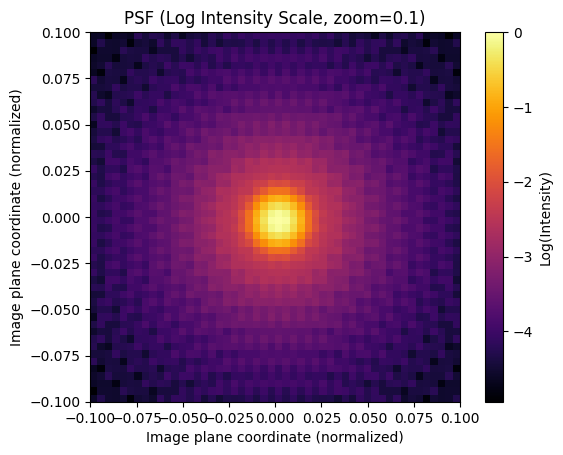
\includegraphics[width=0.45\textwidth]{../images/wave_optics_aberration.png}
    \caption{Wave optics simulation showing PSF distortion and off-axis interference patterns due to lens aberrations.}
    \label{fig:wave-aberration}
\end{figure}

\subsection{Discussion}

The results of the simulations reinforce the theoretical predictions we established earlier.
In the diffraction-limited imaging scenario, ray optics successfully predicted the focal point, yet failed to capture
the spreading of light caused by diffraction. Wave optics, in contrast, clearly visualised the Airy disk and the limited imaging resolution.

In the second scenario, ray optics again captured the geometric origin of aberrations, including the misalignment of
off-axis rays. However, the wave optics model revealed additional information, such as interference-induced
asymmetries and intensity deviations, which are important to understanding how aberrations degrade contrast and quality.

Ultimately, ray optics provided useful qualitative insights and remains valuable for initial optical design and intuition.
However, wave optics offered a more complete and physically accurate representation of the optical systems, especially
when modeling phenomena such as diffraction and aberrations. This validates the necessity of employing wave-based models
in high-resolution or precision imaging applications.
\end{multicols}
{\color{gray}\hrule}
\begin{center}
\section{Conclusions}
\bigskip
\end{center}
{\color{gray}\hrule}
\begin{multicols}{2}
The study explored two optical models, ray optics and wave optics, in the context of imaging systems, through simulation setups
of diffraction and aberration scenarios. Ray optics provide a simplified and intuitive estimate of image formation, operating
under the paraxial approximation, which correctly illustrates focal convergence and spherical aberration effects under ideal
assumptions. On the other hand, wave optics showed a more accurate picture by including diffraction and interference, which ray
optics neglects. The simulation of a point source provided an Airy disk, which reflected the resolution limits due to aperture
diffraction. In the aberration case, a wave model captured asymmetric distortions in the PSF that ray models could not fully
describe. Overall, ray optics is useful for fast approximation and conceptual insight; wave optics is essential for accurate
analysis in systems where diffraction and phase effects are non-negligible. Their combined use offers a deeper understanding of
image formation and the physical limits of optical systems.

\end{multicols}

All work files are available in the GitHub repository: \url{https://github.com/abdullah-qal/optics-project}

\end{document}